\documentclass[12pt]{article}
\usepackage{times} 			% use Times New Roman font

\usepackage[margin=1in]{geometry}   % sets 1 inch margins on all sides
\usepackage{hyperref}               % for URL formatting
\usepackage[pdftex]{graphicx}       % So includegraphics will work
\setlength{\parskip}{1em}           % skip 1em between paragraphs
\usepackage{indentfirst}            % indent the first line of each paragraph
\usepackage{datetime}
\usepackage[small, bf]{caption}
\usepackage{listings}               % for code listings
\usepackage{xcolor}                 % for styling code
\usepackage{multirow}
\usepackage{float}
\usepackage{enumitem}

%New colors defined below
\definecolor{backcolour}{RGB}{246, 246, 246}   % 0xF6, 0xF6, 0xF6
\definecolor{codegreen}{RGB}{16, 124, 2}       % 0x10, 0x7C, 0x02
\definecolor{codepurple}{RGB}{170, 0, 217}     % 0xAA, 0x00, 0xD9
\definecolor{codered}{RGB}{154, 0, 18}         % 0x9A, 0x00, 0x12

%Code listing style named "gcolabstyle" - matches Google Colab
\lstdefinestyle{gcolabstyle}{
  basicstyle=\ttfamily\small,
  backgroundcolor=\color{backcolour},   
  commentstyle=\itshape\color{codegreen},
  keywordstyle=\color{codepurple},
  stringstyle=\color{codered},
  numberstyle=\ttfamily\footnotesize\color{darkgray}, 
  breakatwhitespace=false,         
  breaklines=true,                 
  captionpos=b,                    
  keepspaces=true,                 
  numbers=left,                    
  numbersep=5pt,                  
  showspaces=false,                
  showstringspaces=false,
  showtabs=false,                  
  tabsize=2
}

\lstset{style=gcolabstyle}      %set gcolabstyle code listing

% to make long URIs break nicely
\makeatletter
\g@addto@macro{\UrlBreaks}{\UrlOrds}
\makeatother

% for fancy page headings
\usepackage{fancyhdr}
\setlength{\headheight}{13.6pt} % to remove fancyhdr warning
\pagestyle{fancy}
\fancyhf{}
\rhead{\small \thepage}
\lhead{\small HW1, Adeniran}  % EDIT THIS, REPLACE # with HW number
\chead{\small CS 532, Spring 2021} 

%-------------------------------------------------------------------------
\begin{document}

\begin{centering}
{\large\textbf{HW 1 - Web Science Intro}}\\ % EDIT THIS
                                % REPLACE # with HW num and ADD title
Adeniran Adeniyi\\                     % EDIT THIS
Sunday, Feb 7th 2021  by 11:59pm\\                      % EDIT THIS
\end{centering}

%-------------------------------------------------------------------------

% The * after \section just says to not number the sections

\section*{Q1}
\emph{Consider the "bow-tie" structure of the web in the Broder et al. paper \href{http://snap.stanford.edu/class/cs224w-readings/broder00bowtie.pdf}{"Graph Structure in the Web"} that was described in Module 1.} 

Now consider the following links:
\begin{lstlisting}[language= Python]
A --> B
A --> M
B --> C
C --> A
C --> D
C --> G
E --> F
F --> E
G --> C
G --> H
G --> J
H --> G
I --> H
I --> K
K --> J
L --> D
N --> M
O --> A
O --> P
\end{lstlisting}
\emph{ Draw the resulting 
\href{https://en.wikipedia.org/wiki/Directed_graph}{directed graph} (either sketch on paper or use another tool) showing how the nodes are connected to each other and include an image in your report. This does not need to fit into the bow-tie type diagram, but should look more similar to the graph on slide 24 from}
\href{https://docs.google.com/presentation/d/178GkNtFAPB5fzs1D-wdCnlOdbcTyhpAIz_wKxVUaHVk/edit#slide=id.ga9773ac230_0_799}{ Module-01 Web-Science-Architecture.} 

\emph{For the graph, list the nodes (in alphabetical order) that are each of the following categories:
}
\emph{You may copy the question into your report, but make sure that you make it clear where the question ends and your answer begins.} 
% \par\null\par
% \medskip
% \bigskip
\newline
\newline
\newline
\newline
\begin{itemize}
    \item SCC:
    \item IN:
    \item OUT:
    \item Tendrils:
        \begin{list}{$\circ$}
            \item indicate if the tendril is reachable from IN or can reach OUT
        \end{list}
    \item Tubes:
        \begin{list}{$\circ$}
            \item explain how the nodes serve as tubes
        \end{list}
\end{itemize}
\subsection*{Answer}

% \emph{All figures must have a caption and must be referenced in the text. Example below.}
\begin{figure}[H]
    \centering
    % trim and clip are used to crop the image, trim=left bottom right top
    % width sets max width, height will be scaled appropriately
    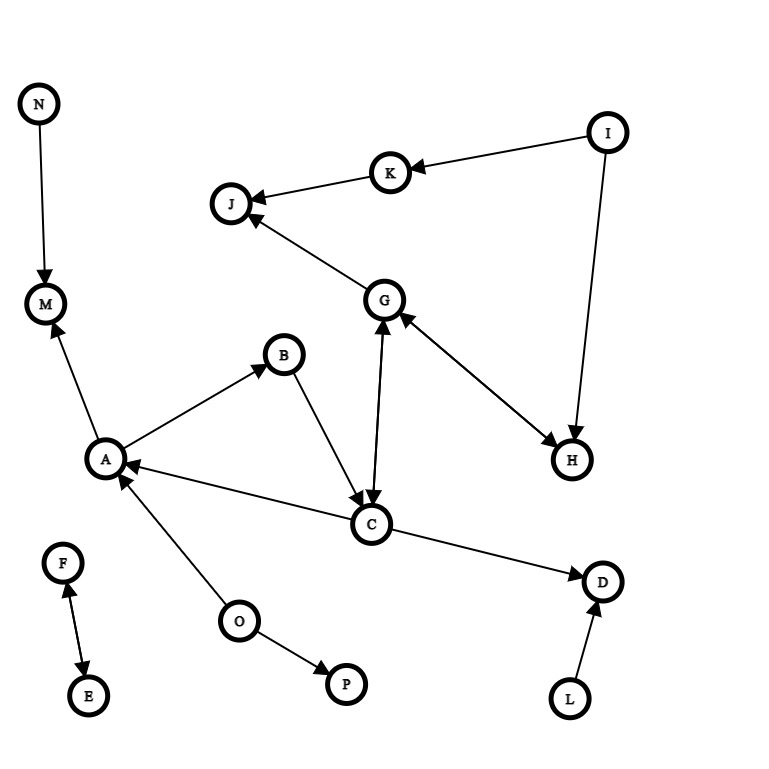
\includegraphics[trim=0 10 0 80, clip, width=\textwidth] {graph.png}
    \caption{Directed graph Question 1 }
    \label{fig:direct graph}
\end{figure}

\begin{itemize}
    \item SCC: A, B, C, G, H
    \item IN: O, I
    \item OUT: M, D, J
    \item Tendrils: N, L, P
    \item Tubes: K
    \item Disconnected: E, F
\end{itemize}
\subsection*{Discussion}

\emph{I followed these instruction below:}
\begin{itemize}
    \item IN: Pages with no in-links or in-links from IN pages and out-links to pages in IN, SCC, Tendrils, or OUT (via a Tube)
    \item SCC: Pages with in-links from IN or SCC and out-links to OUT or SCC. There exists some path of links from every page in SCC to
every other page in SCC
    \item OUT: Pages with no out-links or out-links to other pages in OUT, and all in-links come from OUT, SCC, Tendrils, or Tubes.
    \item Tendrils: Pages that can only be reached from IN or have only out-links to OUT.
    \item Disconnected: Pages that have no in-links from any other components and no out-links to other components. These pages
may be linked to each other.
\end{itemize}

\section*{Q2}
\emph{Demostrate that you know how to use curl and are familiar with the available options. \\
URL to request: \url{http://www.cs.odu.edu/~mweigle/courses/cs532/ua_echo.php}
}
\begin{enumerate}[label=(\alph*)]
    \item First, load the URI directly in your browser and take a screenshot. The resulting webpage should show the User-Agent HTTP header that your web browser sends to the web server.
    \item In a single curl command, request the URI, show the HTTP response headers, follow any redirects, and change the User-Agent HTTP request field to "CS432/532". Show command you used and the result of your execution on the command line. (Either take a screenshot of your terminal or copy/paste into a code segment.)
    \item  Then make the same request again, but without showing the HTTP response headers and with saving the HTML output to a file (i.e., change the options you provide to the curl command). Show the command you used and the result of your execution on the command line. View the HTML output file that was produced by curl in a web browser and take a screenshot.
\end{enumerate}
\emph{Explain the results you get for each of these steps.}
\subsection*{Answer}
\emph{(a)}
\begin{figure}[H]
    \centering
    % trim and clip are used to crop the image, trim=left bottom right top
    % width sets max width, height will be scaled appropriately
    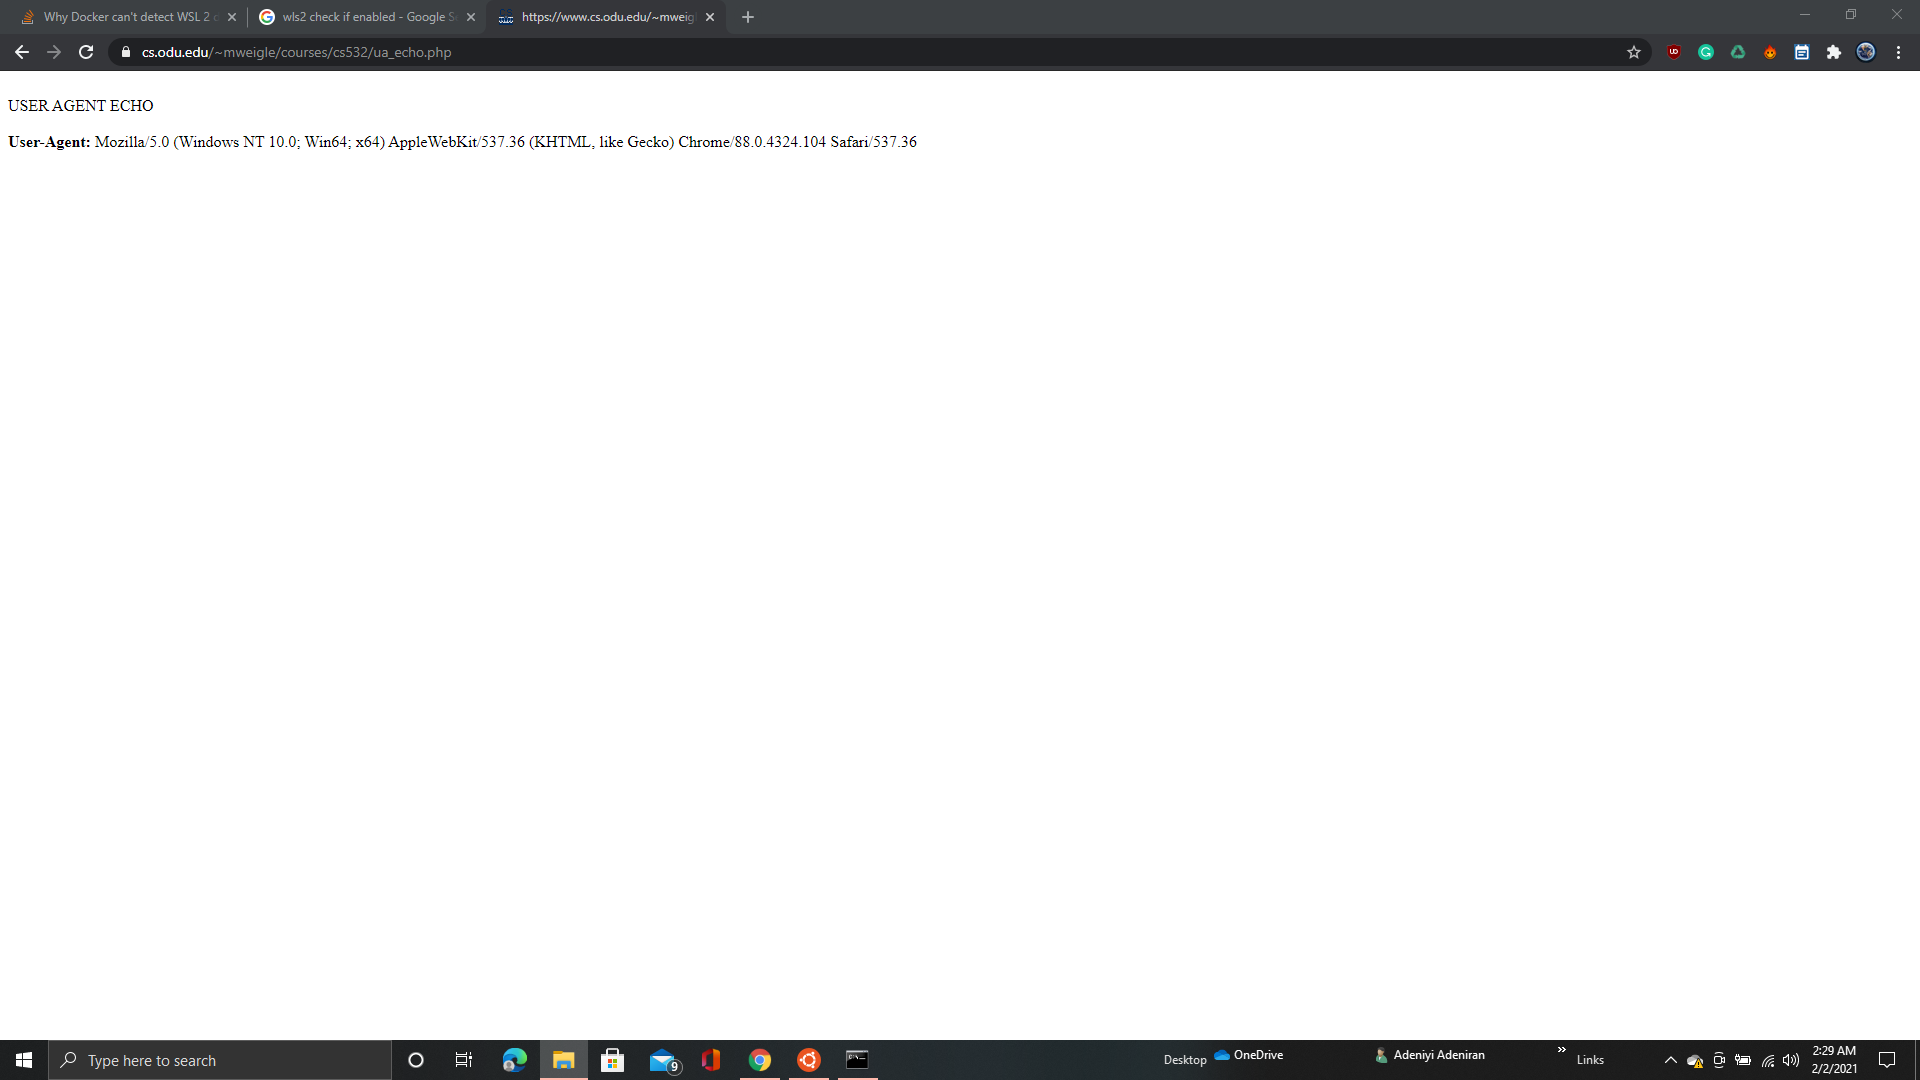
\includegraphics[trim=0 10 0 50, clip, width=\textwidth] {browser.png}
    \caption{Question 2(a)  URL in Browser output}
    \label{fig:browser}
\end{figure}
\subsection*{Discussion}
\emph{The User Agent displayed on the browser after clicking the \url{ http://www.cs.odu.edu/~mweigle/courses/cs532/ua_echo.php} took me to a new webpage that displayed the output shown bellow. \\User-Agent: Mozilla/5.0 (Windows NT 10.0; Win64; x64) AppleWebKit/537.36 (KHTML, like Gecko) Chrome/88.0.4324.146 Safari/537.36}

\emph{(b)}

\begin{lstlisting}
    curl --head -L http://www.cs.odu.edu/~weigle/courses/cs532/ua_echo.php --next -A "CS432/532" http://www.cs.odu.edu/~mweigle/cs532/ua_echo.php
\end{lstlisting}
\begin{lstlisting}
HTTP/1.1 301 Moved Permanently
Server: nginx
Date: Sat, 06 Feb 2021 17:59:48 GMT
Content-Type: text/html
Content-Length: 178
Connection: keep-alive
Location: https://www.cs.odu.edu/~weigle/courses/cs532/ua_echo.php

HTTP/1.1 302 Found
Server: nginx
Date: Sat, 06 Feb 2021 17:59:49 GMT
Content-Type: text/html; charset=utf-8
Content-Length: 0
Connection: keep-alive
Allow: GET, HEAD, OPTIONS
Location: https://www.cs.odu.edu
Referrer-Policy: same-origin
X-Content-Type-Options: nosniff
X-Frame-Options: DENY

HTTP/1.1 301 Moved Permanently
Server: nginx
Date: Sat, 06 Feb 2021 17:59:50 GMT
Content-Type: text/html
Content-Length: 178
Connection: keep-alive
Location: https://odu.edu/compsci

HTTP/1.1 200 OK
Date: Sat, 06 Feb 2021 17:59:51 GMT
Server: Apache/2.4.6 (Red Hat Enterprise Linux)
Vary: Host
X-Content-Type-Options: nosniff
X-Frame-Options: SAMEORIGIN
Connection: close
Content-Type: text/html; charset=UTF-8
Set-Cookie: BIGipServerWEB_HTTPS_PROD.app~WEB_HTTPS_PROD_pool_int=rd741o00000000000000000000ffff8052619eo80; path=/; Httponly; Secure

<html>
<head><title>301 Moved Permanently</title></head>
<body bgcolor="white">
<center><h1>301 Moved Permanently</h1></center>
<hr><center>nginx</center>
</body>
</html>
\end{lstlisting}
\subsection*{Discussion}
\emph{I Entered the command on the terminal area}
\begin{lstlisting}
   curl --head -L http://www.cs.odu.edu/~weigle/courses/cs532/ua_echo.php --next -A "CS432/532" http://www.cs.odu.edu/~mweigle/cs532/ua_echo.php
\end{lstlisting}
\emph{Where -A stands for user-agent $<$name$>$ Send User-Agent $<$name$>$ to server according to curls help command "curl --help". This allows me to specify a custom user agent which I used "CS432/532" as a  substitute. I used the option "-L" which is usually called location is to make curl follow redirects. The --next is used to execute another command in one. The user-agent for both is different. This first one used curl/7.68.0 while the other connection used CS432/532. The --head option displays the header}

\emph{(c)}
\begin{lstlisting}
curl -L http://www.cs.odu.edu/~weigle/courses/cs532/ua_echo.php --next -A "CS432/532" http://www.cs.odu.edu/~mweigle/cs532/ua_echo.php -o index.html
\end{lstlisting}
\begin{figure}[H]
    \centering
    % trim and clip are used to crop the image, trim=left bottom right top
    % width sets max width, height will be scaled appropriately
    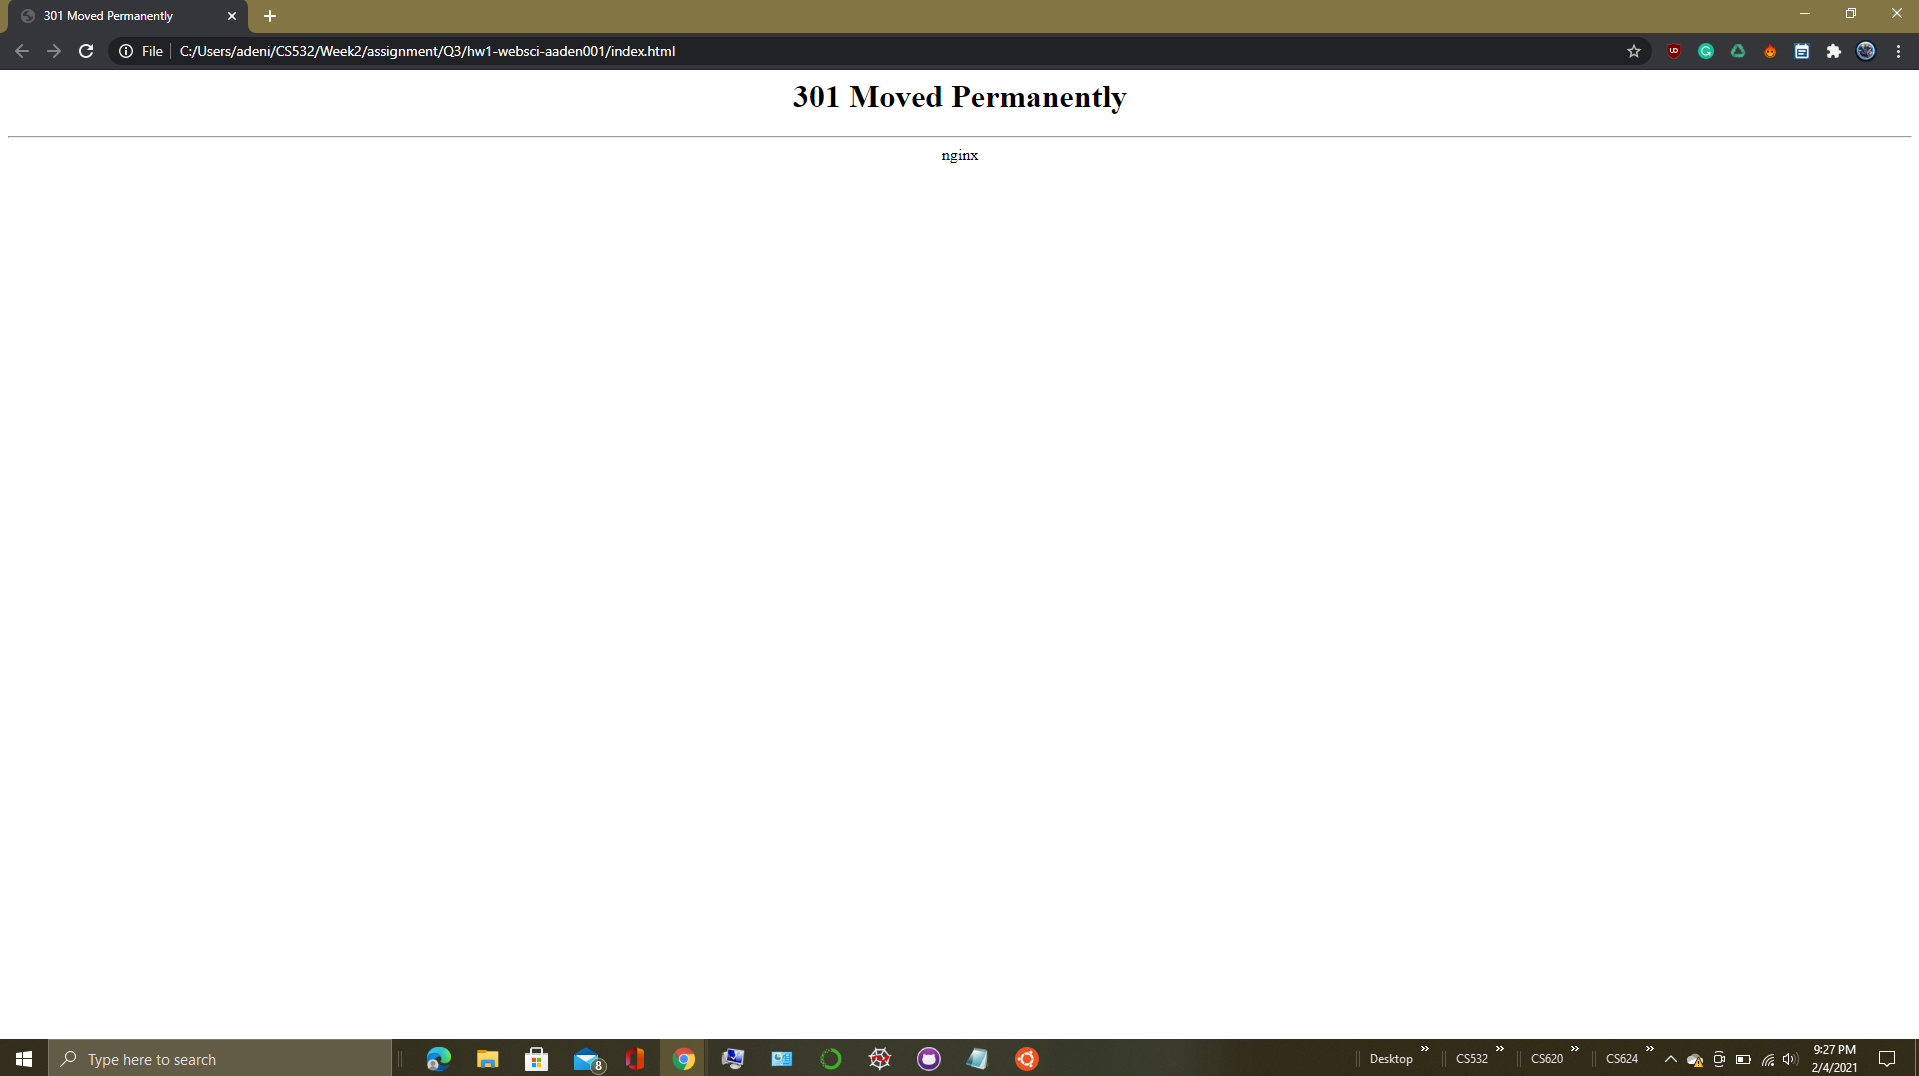
\includegraphics[trim=0 0 0 0, clip, width=\textwidth] {Q2c.png}
    \caption{Question 2(c) output file in a the web browser }
    \label{fig:output file}
\end{figure}
\subsection*{Discussion}
\emph{The input command used to write the output to a .html format to so it can be viewed in the browser. }
\begin{lstlisting}
curl -L http://www.cs.odu.edu/~weigle/courses/cs532/ua_echo.php --next -A "CS432/532" http://www.cs.odu.edu/~mweigle/cs532/ua_echo.php -o index.html
\end{lstlisting}
\emph{I used -o to write to a file and gave the file name to be created and written to}



\section*{Q3}
\emph{Write a Python program to find links to PDFs in a webpage.\\Your program must do the following:}
\begin{itemize}
    \item take the URI of a webpage as a command-line argument
    \item extract all the links from the page
    \item for each link, request the URI and use the Content-Type HTTP response header to determine if the link references a PDF file
    \item for all links that reference a PDF file, print the original URI (found in the source of the original HTML), the final URI (after any redirects), and the number of bytes in the PDF file. (Hint: Content-Length HTTP response header)
\end{itemize}
\subsection*{Answer}

%Importing code from file
\lstinputlisting[language=Python, caption=Python sample code loaded from file, label=lst:import,firstline=1,lastline=77]{pdfLink.py}
% \emph{All figures must have a caption and must be referenced in the text. Example below.}
\begin{figure}[H]
    \centering
    % trim and clip are used to crop the image, trim=left bottom right top
    % width sets max width, height will be scaled appropriately
    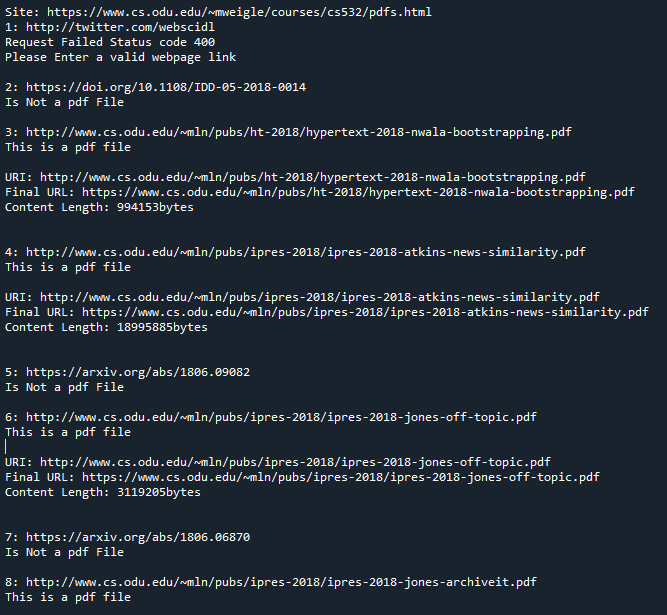
\includegraphics[trim=0 0 0 0, clip, width=\textwidth] {Q3output.png}
    \caption{Sample Output display }
    \label{fig:Q3output}
\end{figure}
\subsection*{Discussion}
\emph{(1) This allows you to run as many arguments supplied to the program as a pretty output display}
\lstinputlisting[language=Python, caption= The drive for the code: , label=lst:import,firstnumber=72,firstline=72,lastline=77]{pdfLink.py}
\emph{(2) Getting necessary libraries that will be used for the task}
\lstinputlisting[language=Python, caption=Python libraries used, label=lst:import,firstnumber=8,firstline=8,lastline=12]{pdfLink.py}
\emph{(3) Request and Beautiful soup libraries. }
\emph{ Line 41 function,}
\lstinputlisting[language=Python, label=lst:import,firstnumber=41,firstline=41,lastline=41]{pdfLink.py}
\lstinputlisting[language=Python, label=lst:import,firstnumber=45,firstline=45,lastline=45]{pdfLink.py}
\lstinputlisting[language=Python, label=lst:import,firstnumber=49,firstline=49,lastline=49]{pdfLink.py}
\lstinputlisting[language=Python, label=lst:import,firstnumber=52,firstline=52,lastline=52]{pdfLink.py}
\emph{takes the url supplied from the command line interface. It makes a get request using the request library. The request is then parsed as a text along with "html parser" as parameters. With this result in soup variable we can get all  href values in each html a tags.}

\emph{(4) Constructing Absolute path, avoiding duplicates and storing}
\lstinputlisting[language=Python, label=lst:import,firstnumber=55,firstline=55,lastline=60]{pdfLink.py}
\emph{Line 55, using urljoin module from urlllib.parse library. We can be able to construct an absolute path url using the URI supplied from the command line and the href\_tags.The href\_tags contains some URI that are relative. This would convert all absolute URI to absolute path URI and would not affect abosulte path URI in href\_tags. Line 55 also ensures that repeated values are avoid. We do nothing as shown in line 57. In line 60 the value is store in a dictionary }

\emph{(5) Content Type Request function . Line 15 function,}
\lstinputlisting[language=Python, label=lst:import,firstnumber=15,firstline=15,lastline=15]{pdfLink.py}
\lstinputlisting[language=Python, label=lst:import,firstnumber=20,firstline=20,lastline=20]{pdfLink.py}
\lstinputlisting[language=Python, label=lst:import,firstnumber=22,firstline=22,lastline=22]{pdfLink.py}
\emph{Takes a URL and checks to see if content-type matches application/pdf. If there is a match We display the supplied link, links after so many redirection if there is, and the size of the content type in bytes. This is done for every link supplied as can be seen in figure \ref{fig:Q3output}}
\section*{References}


\begin{itemize}
    \item { \url{https://stackoverflow.com/questions/44001007/scrape-the-absolute-url-instead-of-a-relative-path-in-python}}
    \item {\url{https://www.askpython.com/python/dictionary/check-if-key-exists-in-a-python-dictionary}}
    \item {\url{https://requests.readthedocs.io/en/master/user/quickstart/#response-content}}
    \item { \url{https://csacademy.com/app/graph_editor/}}
\end{itemize}

\end{document}

